\documentclass{article}
\usepackage[utf8]{inputenc}
\usepackage{xspace}
\usepackage[top=1.5cm, bottom=1.5cm, left=1.5cm, right=1.5cm]{geometry}
\usepackage{enumitem}
\usepackage{graphicx}
\usepackage{textcomp}
\usepackage{amssymb}
\usepackage{ifsym}
\usepackage{xspace}
\usepackage{amsmath}

\title{Facultad de Ciencias. \\Examen Parcial 2. \\ Fundamentos de Bases de             Datos.}
\author{Arteaga Hernández Alejandro Iabin \and 
        Barocio Gómez Luis Fernando \and 
        Ledesma Granados Roberto Andrés \and
        Castrejón Estrada Juan Carlos}
\date{Entrega 28 de Abril 2020}

\begin{document}

\maketitle

\begin{enumerate}

    %%%%%%%%%%%%%%%%%%%%%%%%Pregunta 1%%%%%%%%%%%%%%%%%%%%%%%%%%%
    \item \textbf{(15 puntos) Conceptos básicos.}
    
    \begin{itemize}
        \item Sean \textbf{R} y \textbf{S} dos relaciones \textbf{sin atributos comunes} (sus esquemas son disjuntos). ¿Por qué la operación \textbf{$R \bowtie S$} es equivalente a la operación \textbf{$R \times S$}? ¿Qué ocurre en el caso opuesto, cuando \textbf{R y S} tienen el \textbf{mismo} esquema?
    
        
        Son equivalentes porque no tienen atributos en común. Al hacer el natural join, se hace un producto cruz de las relaciones, y posteriormente se "unen" los atributos que se llaman igual. Si éstos no existen, simplemente se hace un producto cartesiano.\\ Si R y S tienen el mismo esquema, el natural join crea una relación con las tuplas que son exactamente iguales en ambas relaciones.
        
        \item Sean \textbf{R y S} dos relaciones con el \textbf{mismo esquema} y que tienen \textbf{n y m tuplas}, respectivamente. Indica \textbf{cotas} para la cardinalidad de las siguientes operaciones: $R \cup S, R - S, R \cap S, R \bowtie S, R \bowtie S_c $ y $R \div S$
        \begin{itemize}
           \item $max(n, m) \leq |R\cup S| \leq n+m$.
           \item $0 \leq |R-S| \leq n$.
           \item $0 \leq |R\cap S| \leq min(n, m)$.
           \item $0 \leq |R\bowtie S| \leq m*n$.
           \item $0 \leq |R\bowtie _c S| \leq m*n$.
           \item $0 \leq |R / S| \leq m$.
       \end{itemize}
        
        \item Define los conceptos de \textbf{cardinalidad} y \textbf{grado} de una relación.
        
        La cardinalidad es el número de entidades con los cuales una entidad puede relacionarse mediante
        una relación, los tipos de cardinalidad son: Uno a uno, uno a muchos ó muchos a uno y muchos a muchos, y el grado de una relación es el número de entidades que participan en una relación.
        
        \item ¿Qué restricción impone una \textbf{llave primaria} sobre su relación en un modelo de datos relacional?
        Es única, no nula y todos los elementos de la relación dependen funcionalmente de ella.
        
        \item ¿Qué es una \textbf{llave foránea} y \textbf{qué restricciones} impone el usarla en una base de datos relacional?
        
        Es un atributo que hace referencia a una llave primaria en otra tabla, tiene como restricción
        que para usarla o insertarla, debe existir ese valor como llave primaria en la otra tabla a la
        que hace referencia
        
    \end{itemize}
    %%%%%%%%%%%%%%%%%%%%%%%%Pregunta 2%%%%%%%%%%%%%%%%%%%%%%%%%%%
    \item (10 puntos) Transforma el siguiente \textbf{diagrama E/R} a su equivalente \textbf{Modelo Relacional}: 
    
    
    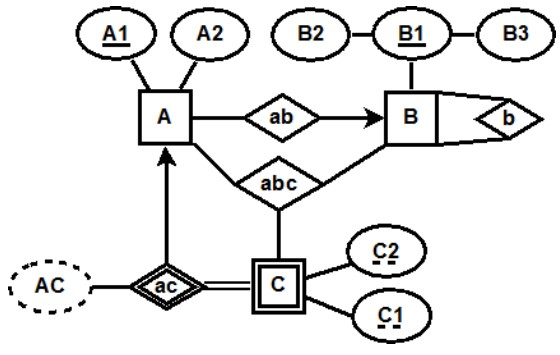
\includegraphics[scale=0.5]{2.jpg}
    
    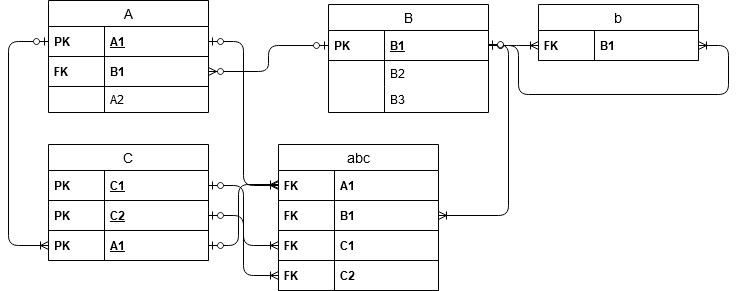
\includegraphics[scale = 0.65]{2_res.png}
    
    
    
    
    %%%%%%%%%%%%%%%%%%%%%%%%Pregunta 3%%%%%%%%%%%%%%%%%%%%%%%%%%%
    \item (15 puntos) Traduce el siguiente esquema al \textbf{Modelo Relacional}.
    
    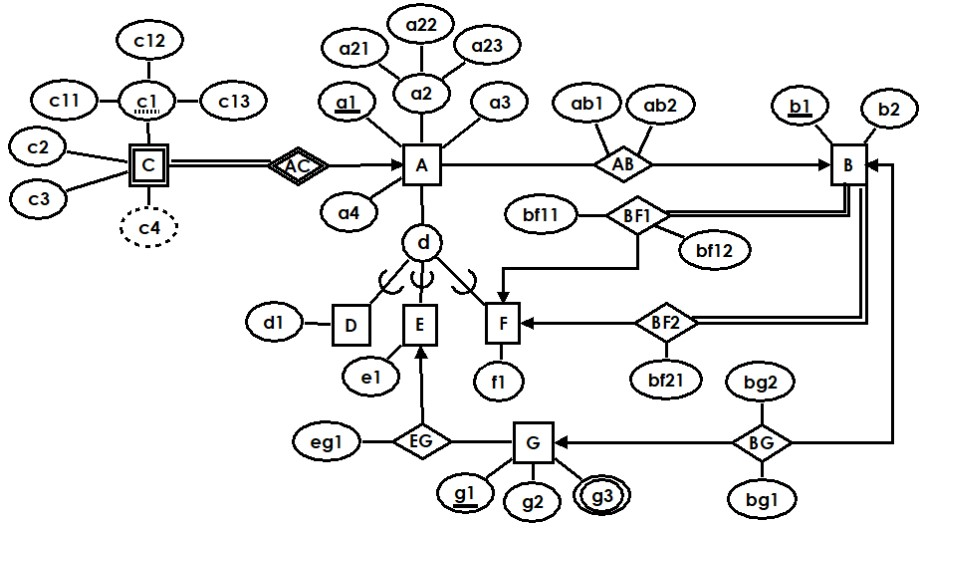
\includegraphics[scale = 0.5]{3.jpg}
    
    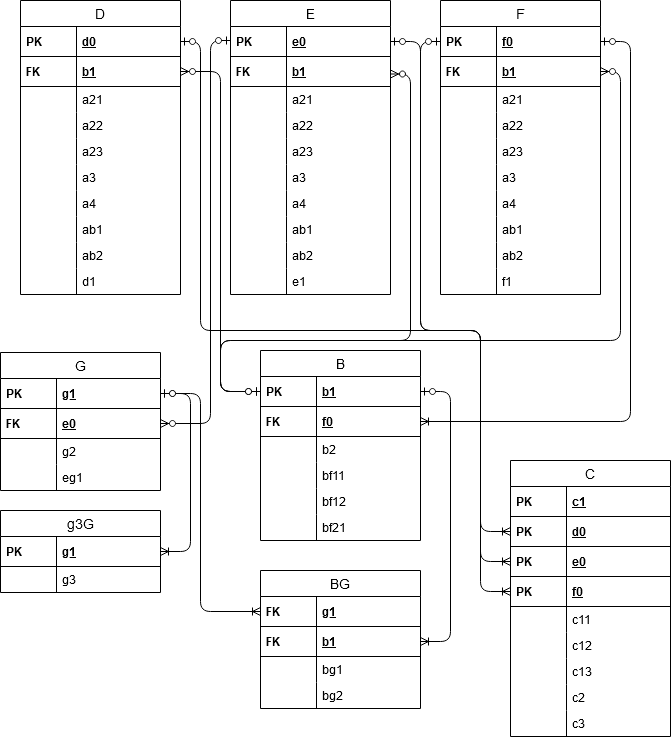
\includegraphics[scale = 0.65]{3_res.png}
    
    
    
    %%%%%%%%%%%%%%%%%%%%%%%%Pregunta 4%%%%%%%%%%%%%%%%%%%%%%%%%%%
    \item (30 puntos) \textbf{Álgebra Relacional}.
    
    Tienes una \textbf{Base de Datos} con el siguiente esquema. Escribe una expresión en álgebra relacional para cada una de las siguientes consultas.
    \begin{itemize}[label={}]
        \item \textbf{Frecuenta} (\underline{bebedor},\underline{bar}, desde)
        \item \textbf{Sirve} (\underline{bar, cerveza})
        \item \textbf{Gusta} (\underline{bebedor, cerveza})
    \end{itemize}
    
    
   \fbox{\begin{minipage}{15em}
    Donde \textbf{Frecuenta} indica si un bebedor frecuenta un bar, \textbf{Sirve} indica si un bar sirve un tipo de cerveza y \textbf{Gusta} indica si un bebedor gusta de un tipo de cerveza.
         \end{minipage}}
    
    \begin{enumerate}
        \item Una lista de los bebedores que frecuentan el bar \textbf{Beer para Creer} desde el \textbf{26 de abril de 1989}. 
        
        $\pi_{bebedor}(\sigma_{bar= Beer para Creer \wedge \text{ desde = 26 de abril de 1989}}(Frecuenta))$
        
        \item Los bebedores que no frecuenten bares con cervezas que les gustan
        
        $s \leftarrow (Sirve \bowtie Gusta)$
        
        $\pi_{bebedor}(Frecuencia \bowtie_{Frecuenta.bar!=s.bar} \wedge_{Frecuencia.bebedor=s.bebedor}\  S)$
        
        \item Encontrar los bares que venden la cerveza \textbf{Duff} pero que no venden \textbf{XX Lager}.
        
        $s \leftarrow \pi_{bar}(\sigma_{cerveza=Duff}(Sirve))$
        
        $p \leftarrow \pi_{bar}(\sigma_{cerveza=XX lager}(Sirve))$
        
        $s-p$
        
        \item Asumiendo que, si existen, una lista con los bares que sirven todas las cervezas
        
        $n \leftarrow Y_{count(cerveza)(\pi_{cerveza}(Sirve))}$
        
        $p \leftarrow_{bar} Y_{count(cerveza)}(Sirve)$
        
        $\pi_{bar}(\sigma_{count=n}(p))$
        
        \item Lista que muestre información de bares que frecuentan los bebedores y las cervezas que les gustan. Mostrar la información agrupada por bar
        
        $barY(Frecuencia \bowtie Gusta)$
        
        \item Lista de los bares que venden la cerveza que más les gusta a los bebedores.
        
        $p \leftarrow_{cerveza}Y_{count(bebedor)}(Gusta)$
        
        $m \leftarrow Y_{max(count)}(p)$
        
        $c \leftarrow \pi_{cerveza}(\sigma{count=m}(p))$
        
        $c \bowtie Sirve$
        
        
        \item Los bares que van a quebrar, pues ningún bebedor los frecuenta.
        
        $s \leftarrow_{bar} Y_{count(bebedor)}(Frecuenta)$
        
        $\pi_{bar}(\sigma_{count=0}(s))$
        
        \item Borrar toda la información de los bares que sirven la cerveza \textbf{Pacífico y Montejo}.
        
        $s \leftarrow \pi(\sigma_{cerveza=Pacifico \vee cerveza=Montejo}(Sirve))$
        
        $Sirve \leftarrow Sirve - s$
        
        $p \leftarrow Frecuencia \bowtie \pi_{bar}(s)$
        
        $Frecuenta \leftarrow Frecuenta -p$
        
        \item Actualizar la información del bar \textbf{La Tapilla Sixtina} ya que, a partir de hoy el bar se llamará \textbf{Bar Veider}
        
        $S \leftarrow \sigma_{bar=\text{Tapilla Sixtina}}(Sirve)$
        
        $p \leftarrow \sigma_{bar=\text{Tapilla Sixtina}}(Frecuencia)$
        
        $Sirve \leftarrow Sirve - s$
        
        $Frecuenta \leftarrow Frecuenta - p$
        
        $Sirve \leftarrow Sirve \cup(\{ Bar Vieder\} \times \pi_{frecuenta}(S))$
        
        $Frecuenta \leftarrow Frecuenta \cup \pi_{bebedor, bar, desde}((\pi_{bebedor, desde}(s) \times \{ Bar Vieder\}))$
        
        
        \item Insertar la información del bar \textbf{BBT Otra}, el cual sirve las siguientes cervezas: \textbf{Negra Modelo, Bohemia} y todas las cervezas que sirve el \textbf{Bar-Tolo}.
        
        $s \leftarrow \pi_{cerveza}(\sigma_{bar=\text(Bar Tolo)}(Sirve))$
        
        $Sirve \leftarrow  Sirve \cup (\{ Bar Tolo \} \times (s \cup \{ \text{Negra Modelo, Bohemia\}}))$
        
    \end{enumerate}
    
    %%%%%%%%%%%%%%%%%%%%%%%%Pregunta 5%%%%%%%%%%%%%%%%%%%%%%%%%%%
    \item (10 puntos) \textbf{Álgebra relacional} 
    
    Tienes la relación \textbf{Producto} (\textbf{\underline{IDArticulo}}, máximo, mínimo, promedio) que registra los precios de venta \textbf{máximo, mínimo} y \textbf{promedio} (históricos) de varios productos que oferta una tienda en línea. Considera la siguiente consulta en álgebra relacional: 
    
    $$P_{1}= \pi_{IDArticulo,maximo} (Producto)\quad;\quad P_2 = \pi_{IDArticulo,minimo}(Producto)$$
    
    $$\rho_{idArt \leftarrow IDArticulo,max \leftarrow maximo}(P_1)\quad ;\quad \rho_{idArt \leftarrow IDArticulo,min \leftarrow minimo}(P_2) $$
    
    $$P_3 = \pi_{idArt}(P_{1}\bowtie_{max<maximo} Producto)\quad ;\quad P_4 = \pi_{idArt}(P_{2} \bowtie_{min>minimo} Producto)$$
    
    $$P_5 = \pi_{IDArticulo}(Producto)-P_3 \quad ; \quad P_6 = \pi_{IDArticulo}(Articulo)-P_4$$
    
    $$Resultado = \pi_{nombreProducto}(Producto \bowtie (P_5 \cup P_6))$$
    
    Explica los puntos más importantes de la consulta anterior e indica qué información se tiene en la relación Resultado, después de realizar todas las expresiones de álgebra relacional.
    \\ \\
    Consideramos que los puntos más importantes del procedimiento son las operaciones para obtener p3 y p4. Las otras operaciones son mucho más elementales, mientras que el join se encarga de obtener los productos que no se quieren tomar en cuenta.\\
    Funciona como sigue: Al hacer p1 $\bowtie$ Producto, estamos haciendo el producto cartesiano de éstas relaciones, ya que no tienen atributos en común. El theta join, se queda entonces con aquellos renglones del producto cartesiano en los que max $<$ maximo. Es decir, únicamente se queda con los productos cuyo precio máximo es menor al máximo global. Algo equivalente sucede para p4, obtenemos los productos cuyo precio mínimo es mayor al mínimo global.
    \\
    Posteriormente, P5 y P6 obtienen los idArticulos de los productos que si tienen como máximo/mínimo el máximo/mínimo global. De forma que la relación Resultado tiene la información de los nombres de los productos que tienen como precio máximo/mínimo el precio global máximo/mínimo.

    
    %%%%%%%%%%%%%%%%%%%%%%%%Pregunta 6%%%%%%%%%%%%%%%%%%%%%%%%%%%
    \item (5 puntos)\textbf{Modelo Relacional}
    
    Un día escuchas a un ingeniero afirmar lo siguiente: \textbf{”…al convertir un modelo E/R que tiene N entidades y M relaciones a un Modelo Relacional equivalente, se obtendrán como máximo N + M relaciones”}. ¿Esta afirmación es correcta? Justifica tu respuesta.
    \\
    \\
    
    
    Esto es falso, un contra ejemplo es el caso cuando una entidad tiene un atributo multivaluado, a ese
    atributo se le genera una tabla con los valores.
    
    Por lo tanto este modelo con 2 entidades y 1 relación tiene 4 relaciones en el modelo relacional y no 3.
    
    \begin{figure}[h]
        \centering
        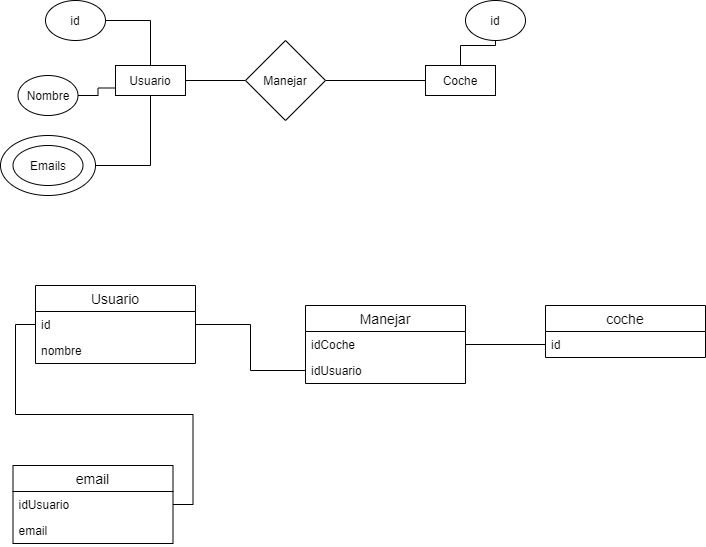
\includegraphics[scale=0.6]{6.png}
        \label{fig:6}
    \end{figure}
    
    
    %%%%%%%%%%%%%%%%%%%%%%%%Pregunta 7%%%%%%%%%%%%%%%%%%%%%%%%%%%
    \item (15 puntos) Sean las relaciones \textbf{R y S} definidas a continuación:
    
    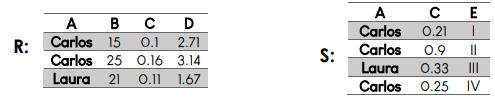
\includegraphics[scale = 1]{7.jpg}
    
    Obtén (o indica por qué es posible obtener) el resultado de las siguientes expresiones:
    
    \begin{enumerate}
        \item $a = R \cup U$
        
        No fue posible obtener resultado porque no coinciden las columnas de la tabla R con la tabla S.
        
        \item $b = \pi_{A,C}(R)$ 
        
            \begin{tabular}{|l|l|}
            \hline
                A      & C    \\ \hline
                Carlos & 0.1  \\ \hline
                Carlos & 0.16 \\ \hline
                Laura  & 0.11   \\ \hline
            \end{tabular}
        
        
        \item $c = \pi_{A,C}(S)$
        
        \begin{tabular}{|l|l|}
        \hline
            A      & C    \\ \hline
            Carlos & 0.21 \\ \hline
            Carlos & 0.9  \\ \hline
            Laura  & 0.33 \\ \hline
            Carlos & 0.25 \\ \hline
        \end{tabular}
        
        \item $d = b \cup c$
        
        \begin{tabular}{|l|l|}
        \hline
            A      & C    \\ \hline
            Carlos & 0.1  \\ \hline
            Carlos & 0.16 \\ \hline
            Laura  & 0.11 \\ \hline
            Carlos & 0.21 \\ \hline
            Carlos & 0.9  \\ \hline
            Laura  & 0.33 \\ \hline
            Carlos & 0.25 \\ \hline
        \end{tabular}
        
        \item $e = b \cap c$
        
        $e =$ \o
        
        \item $f = b-c$
        
        \begin{tabular}{|l|l|}
        \hline
            A      & C    \\ \hline
            Carlos & 0.1  \\ \hline
            Carlos & 0.16 \\ \hline
            Laura  & 0.11 \\ \hline
        \end{tabular}
        
        \item $g = c-d$
        
        \begin{tabular}{|l|l|}
        \hline
            A      & C    \\ \hline
            Carlos & 0.21 \\ \hline
            Carlos & 0.9  \\ \hline
            Laura  & 0.33 \\ \hline
            Carlos & 0.25 \\ \hline
        \end{tabular}
        
        \item $h = \sigma_{C>0.15}(S)$
        
        \begin{tabular}{|l|l|l|}
        \hline
            A      & C    & E   \\ \hline
            Carlos & 0.21 & I   \\ \hline
            Laura  & 0.33 & III \\ \hline
            Carlos & 0.25 & IV  \\ \hline
        \end{tabular}
        
        \item $i=\pi_A(h)$
        
        \{Carlos, Laura\}
        
        \item $j = R \times S$
        
        \begin{tabular}{|l|l|l|l|l|l|l|}
        \hline
            R\_A   & R\_B & R\_C & R\_D & S\_A   & S\_C & S\_E \\ \hline
            Carlos & 15   & 0.1  & 2.71 & Carlos & 0.21 & I    \\ \hline
            Carlos & 15   & 0.1  & 2.71 & Carlos & 0.9  & II   \\ \hline
            Carlos & 15   & 0.1  & 2.71 & Laura  & 0.33 & III  \\ \hline
            Carlos & 15   & 0.1  & 2.71 & Carlos & 0.25 & IV   \\ \hline
            Carlos & 25   & 0.16 & 3.14 & Carlos & 0.21 & I    \\ \hline
            Carlos & 25   & 0.16 & 3.14 & Carlos & 0.9  & II   \\ \hline
            Carlos & 25   & 0.16 & 3.14 & Laura  & 0.33 & III| \\ \hline
            Carlos & 25   & 0.16 & 3.14 & Carlos & 0.25 & IV   \\ \hline
            Laura  & 21   & 0.11 & 1.67 & Carlos & 0.21 & I    \\ \hline
            Laura  & 21   & 0.11 & 1.67 & Carlos & 0.9  & II   \\ \hline
            Laura  & 21   & 0.11 & 1.67 & Laura  & 0.33 & III  \\ \hline
            Laura  & 21   & 0.11 & 1.67 & Carlos & 0.25 & IV   \\ \hline
        \end{tabular}
        
    \end{enumerate}
    
    
\end{enumerate}

\end{document}
